\chapter{Clusterização} \label{cap:clusterizacao}

A clusterização é denominada como técnica para organização ou agrupamento de uma coleção de padrões, ou elementos que sigam padrões, em \textit{clusters} baseada em similaridade.
Trata-se de uma técnica bastante utilizada em análise exploratórias, agrupamentos, tomada de decisão e implementações de \textit{machine learning}, como:
mineração de dados, recuperação de documentos, segmentação de imagens e padronização \cite{clustering_review}.

A aplicação da técnica pode ser resumida nos passos apresentados na Figura \ref{fig:tasks_clustering}.

\begin{figure}[h!]
\centering
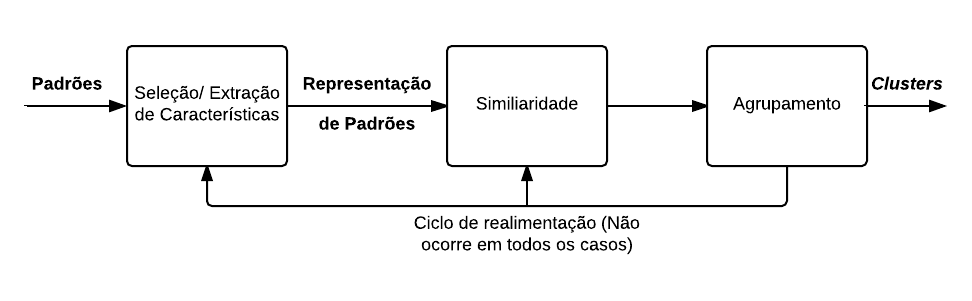
\includegraphics[scale=0.6]{figuras/tasks_clustering.png}
\caption{Passos para clusterização. Adaptado de \citeonline{clustering_review}}
\label{fig:tasks_clustering}
\end{figure}

A representação de padrões está relacionada ao número de classes, número de padrões disponíveis e o número, tipo e escala
das características disponíveis no algoritmo de clusterização. Algumas dessas informações podem não ser controladas pelos
profissionais \cite{clustering_review}.

A seleção de características é o processo de identificação do subconjunto das características mais eficaz para a clusterização, já a extração
de características é o uso de uma ou mais transformações das características de entrada para produzir novas características \cite{clustering_review}.

A similaridade, em geral, é medida por uma função de distância entre um par de padrões ou elementos. Essa função de distância pode variar
de acordo com o contexto da aplicação. E por fim, o agrupamento pode ser realizado com uso de vários algoritmos diferentes \cite{clustering_review}.

\section{Análise de \textit{clusters}}

\citeonline{tan2013data} definem a análise de \textit{clusters} como a ação que agrupa objetos de dados baseado apenas nas informações contidas
nos dados do próprio objeto que permitam descrever os objetos e suas relações. 

Classificação é o processo de encontrar um modelo que possa descrever e distinguir classes de dados \cite{han2011data}.

\citeonline{tan2013data}, \citeonline{han2011data} ressaltam a diferença entre classificação supervisionada e classificação não supervisionada.
Na classificação supervisionada os objetos de dados são analisados a partir de rótulos de classe predefinidos nos objetos, ou seja, 
com as classes de dados previamente definidas e conhecidas. \citeonline{han2011data} chamam este tipo de dado de "dado treinado"
(dados cujos rótulos são conhecidos), onde o modelo que o descreve é obtido a partir da análise dos rótulos.
Na classificação não supervisionada, os rótulos de classe são obtidos a partir da análise dos dados dos objetos, tão somente \cite{tan2013data}.

A clusterização geralmente se refere a este último tipo de classificação \cite{tan2013data}, onde os rótulos de classes dos objetos podem não existir ainda e 
o método empregado na clusterização pode gerar rótulos para um grupo de dados do conjunto \cite{han2011data}.

Os objetos são agrupados (ou "clusterizados") buscando maximizar a similaridade intraclasse e minimizar a similaridade interclasse.
Em outras palavras, o objetivo é formar \textit{clusters} cujos elementos tenham alta similaridade entre si em um mesmo \textit{cluster} 
e baixa similaridade a elementos de outros \textit{clusters} \cite{han2011data}. Por fim, um \textit{cluster} pode ser visto como uma
classe de objetos de onde se é possível derivar regras para o grupo \cite{han2011data}.

Apesar de parecer lógico e simples querer maximizar a similaridade intraclasse e minimizar a similaridade interclasse entre um conjunto de dados, 
\citeonline{tan2013data} exemplificam o quão difícil esta tarefa pode ser na Figura \ref{fig:clusters_difficulty}, onde temos um conjunto
de pontos (a) que pode ser agrupado de formas diferentes gerando quantidades diferentes de \textit{clusters} (b, c, d).

\begin{figure}[h!]
\centering
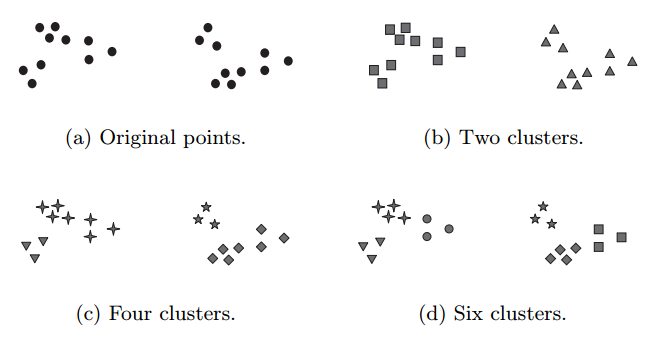
\includegraphics[scale=0.4]{figuras/clusters_difficulty.png}
\caption{Formas de se agrupar o mesmo conjunto de dados. Fonte: \cite{tan2013data}}
\label{fig:clusters_difficulty}
\end{figure}

 
\section{Tipos de clusterização}

\section{Algoritmos de clusterização}